\part{Tudo sobre senhas}

\section{Introdução do Capítulo}

Neste capítulo vamos falar sobre uma das principais formas de proteger seus conteúdos no meio digital: as senhas. Vamos falar sobre como elas funcionam, o que elas são, como criá-las e armazená-las.

\chapter{Como Funcionam as senhas}

A senha é apenas uma das formas de acesso a um conteúdo restrito. Eles são classificados em: Algo que a pessoa possui; Algo que a pessoa é; e algo que a Pessoa Sabe. Algo que a pessoa possui é um objeto físico que se traduz digitalmente para garantir algum acesso, exemplos são Cartões de Banco, Crachás, ou tokens de acesso. Algo que a pessoa é são elemento físicos biométricos para acesso, como sensor de digitais dos dedos, ou de voz. Por fim, temos Algo que a Pessoa sabe, este é um conhecimento combinado para o acesso que se manifesta em perguntas pré-definidas, mas principalmente em senhas.
\begin{figure}[h]
\centering
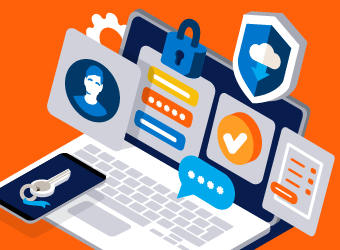
\includegraphics{img/formas_de_acesso.png}
\end{figure}

As Senhas portanto são chaves para acesso a determinado ambiente virtual ou físico restrito, ou então códigos que permitem a decodificação de alguma criptografia por meio de um conhecimento específico de alguma pessoa.

O funcionamento de senhas em si funciona a partir de uma equivalência de caracteres armazenados por um registro feito anteriormente com os caracteres fornecidos quando se tenta acessar um ambiente restrito. Estes caracteres podem ser do alfabeto (a, A, z, Z), Numéricos (1, 3, 0), ou caracteres especiais (*, \&, \#). Uma vez que há um número limitado de caracteres existentes para se criar senha e também um tamanho limite de caracteres para se fazer uma senha, há a possibilidade da senha ser descoberta por alguém que não a criou se todas as possibilidades forem tentadas a exaustão. A isso, damos o nome de ataque de força bruta. Este ataque normalmente é feito com um programa de computador tentando todas as combinações possíveis de caracteres e sua quantidade nas senhas. É muito mais comum que as senhas sejam feitas apenas com letras, ou letras e números, reduzindo-se a complexidade delas, fica mais fácil a descoberta a partir do ataque de força bruta. Portanto quando se utiliza letras, números e caracteres especiais a segurança da senha é aumentada. O cálculo para a descoberta de uma senha por ataque de força bruta.

Façamos os cálculos da quantidade de possibilidades de senhas:
Com uma senha com número \textit{n} de caracteres e a ordem dos caracteres importarem devemos calcular a quantidade de possibilidades de senhas (\textit{s}) com o número de caracteres exponenciado à quantidade de caracteres (\textit{q})
\[s = n ^q\]
Para comparação podemos usar uma senha com 8 caracteres.
Considerando-se uma senha apenas de letras: Temos 26 letras no alfabeto, porém caracteres maiúsculos e minúsculos são considerados diferentes então temos \(26 . 2 = 52 \) teremos então \(s = 52^8 = 5,3 . 10^{13} \) de possibilidades de senhas a serem feitas, ou seja 53 trilhões de possibilidades. Um algoritmo de Força Bruta resolve essas tentativas em 49 minutos.

Quando adicionamos números teremos mais 10 caracteres então \( 10 + 52 = 62 s = 62^8 = 2,8 . 10^{14} \) 218 trilhões de possibilidades, com um algoritmo de Força Bruta o tempo de resolução sobe para 4 horas.

\begin{figure}[h]
\centering
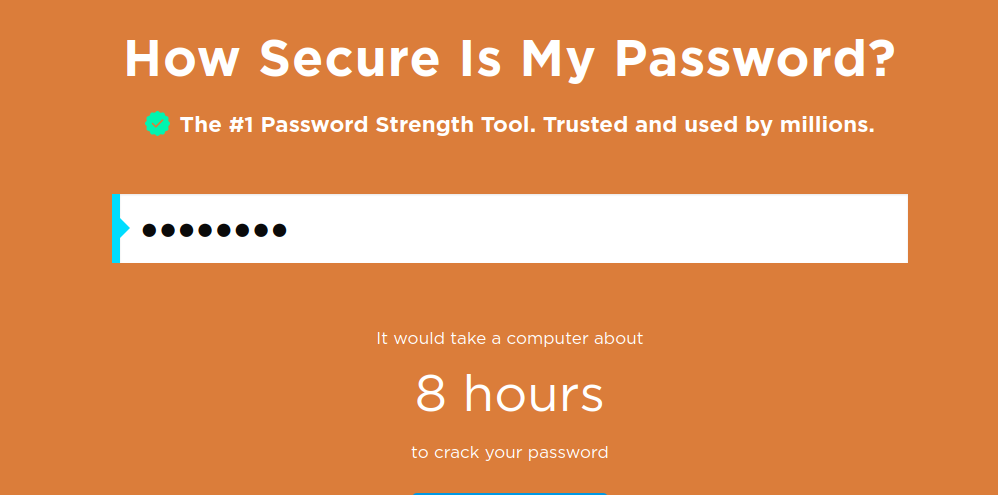
\includegraphics[width=\textwidth]{img/tempo_decifrar_senha.png}
\end{figure}


Adicionando-se a isso os caracteres especiais colocamos à soma mais 30 caracteres. \( 30 + 62 = 92 s = 92^8 = 6,6 . 10^{15} \) 6,6 quatrilhões, resultando em um tempo de 5 dias para se conseguir a senha em um algoritmo de força bruta.

Notamos uma boa diferença na segurança da senha adicionando todos os tipos possíveis de caracteres, mas também aumentando o número de caracteres temos um grande aumento de segurança. No caso de uma senha só com letras temos um aumento de 49 minutos de resolução para 92 dias de resolução utilizando 10 caracteres, ao invés de 8. Analisando uma senha com todos os tipos de caracteres temos um tempo de 5 dias de resolução com 8 caracteres e 105 anos para resolver com 10 caracteres.

/(Adicionar tabela aqui)

Porém esta não é a única forma de se conseguir descobrir uma senha. Outro ataque comum à segurança de senhas é o chamado Ataque de Dicionário que usa um banco de palavras para tentar encaixar nas tentativas exaustivas de correspondência com a senha. Tal tipo de ataque fragiliza senhas que usam as palavras mais comumente usadas em senhas extraídas de bancos de dados comprometidos e também de forma mais pessoal fica mais frágil utilizar informações pessoais facilmente encontradas de forma pública, uma nome de filho, animal de estimação, time que torce ou datas especiais podem ser utilizadas para tornar um Ataque de Dicionário mais eficiente.

\section{Formas de Autenticação Mistas}
\begin{figure}[h]
\centering
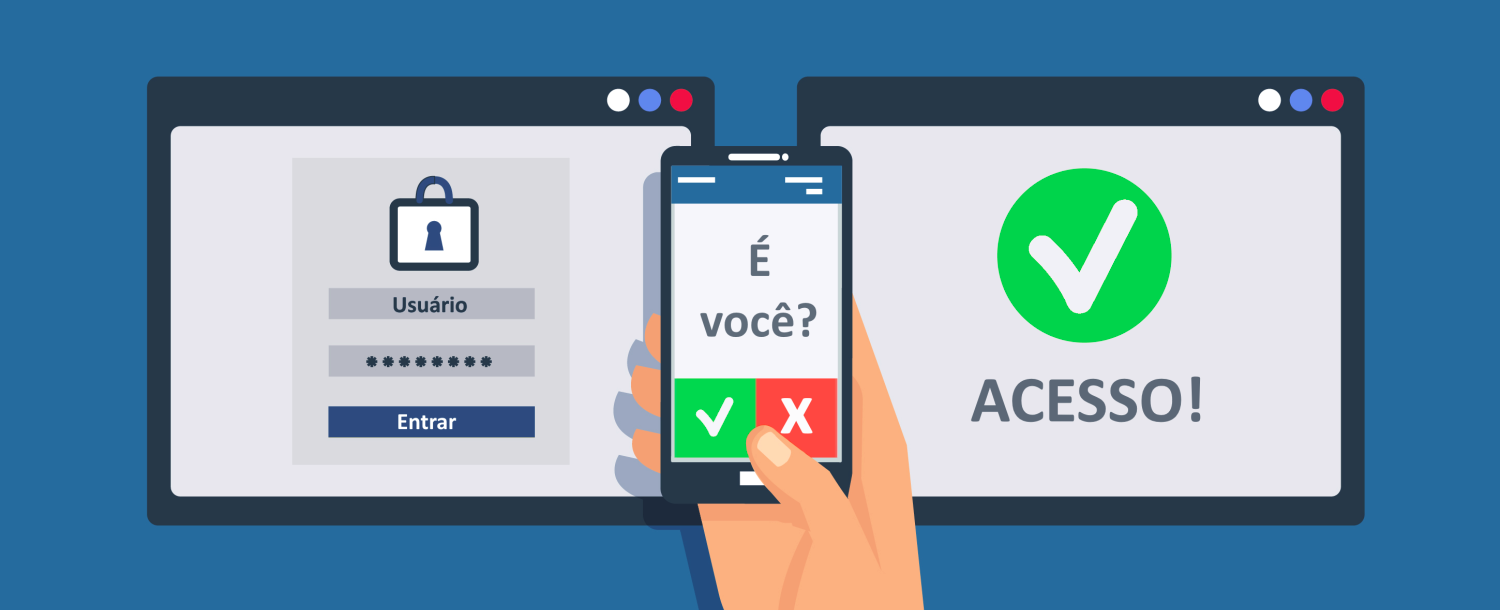
\includegraphics[width=\textwidth]{img/multipla_autenticacao.png}
\end{figure}

Considerando a quantidade de ataques e a necessidade da Segurança da Informação de sempre se aprimorar, a forma de autenticação da identidade apenas por senha, ou seja, algo que o usuário sabe. Para trazer maior segurança passou-se a utilizar modos de autenticação combinados. Desse modo se aumenta a segurança de acessos mais sensíveis ,um bom exemplo é uma conta de banco no celular que não utiliza apenas sua senha, ela utiliza também um celular que a pessoa tenha informado e repassa um código de uso único para o número informado. Essa abordagem é realizada por um número cada vez maior de empresas, mas muitas vezes é preciso ser adotado pelo usuário ainda, o que é muito recomendável de ser feito para acessos delicados, como aqueles que realizam acesso a pagamentos e informações sensíveis.
\begin{ficadica}
    Nas aplicações mais importantes é sempre recomendável adicionar pelo menos 2 formas de autenticação diferentes
\end{ficadica}


\section{Criando e Armazenando Senhas}
A partir desta noção de funcionamento de senhas e de algumas maneiras que elas podem ser descobertas, podemos pensar sobre como manter um acesso de autenticação por senha seguro. Primeiro devemos saber como criar uma senha boa. Depois devemos pensar que hoje em dia criamos cada vez mais senhas para uma infinidade de acessos que precisamos realizar, surge então o questionamento de como lembrar de todas as senhas, se elas devem ser diferentes ou não.

\subsection{Criando Senhas}
O modo como se deve escolher uma senha não é uma unanimidade atualmente. Mas á boas dicas do que não se deve fazer ao criar uma senha e o que se deve fazer como pressuposto básico.

\begin{ficadica}
\textbf{Como não se deve fazer uma senha:}
\begin{itemize}
    \item Não use seu próprio nome, ou o nome do usuário
    \item Não use dados pessoais
    \item Não use nomes próprios
    \item Não use uma sequência de caracteres como "123" ou "abc" ou até "qwerty"
\end{itemize}
\end{ficadica}

\begin{ficadica}
\textbf{Dicas para fazer uma senha:}
\begin{itemize}
    \item Utilize Caracteres do alfabeto com letras maiúsculas e minúsculas
    \item Utilize todos os tipos de caracteres: Letras, Números e Caracteres Especiais
    \item Utilize pelo menos 8 caracteres
\end{itemize}
\end{ficadica}

Seguindo estas dicas há caminhos que podem ser tomados na criação de uma senhas: 

Podem ser criadas senhas de modos aleatórios que trazem alta segurança mas uma difícil memorização. Como por exemplo: Lgaao9l1W80jdOS.

Mas também podem ser criadas senhas que não consideram alguns tipos de ataque, como o ataque de dicionário mas possuem segurança por seus tipos de caracteres e tamanho, e trazem uma facilidade melhor para memorizar. Exemplo: Caixa4Fortificada!

\subsection{Armazenando Senhas}

Bom, além da criação das senhas também é importante pensar sobre como se lembrar delas, sendo que cada vez mais se faz a necessidade da criação de diversas contas de acesso diferentes pela internet. Pensando nisso, é uma boa ideia usar a mesma senha em várias contas? Não, essa não é uma boa ideia, pois ocasionalmente as empresas que guardam estes dados sofrem vazamentos de informações permitindo que as senhas dos usuários sejam conhecidas publicamente. Isso não ocorre apenas em empresas pequenas, grandes empresas também já sofreram e podem sofrer com um vazamento destes. O que ocorre quando um grande volume de senhas são vazadas ao público são diversas pessoas mau-intencionadas que tentam usá-las em outros serviços que a pessoa possui conta, muitas vezes conseguindo acesso com esta mesma senha.

\begin{atencao}
Um modo de guardar senha muito utilizado é anotando a senha em um papel em algum lugar da sua área de trabalho. Essa prática é causa um grande risco de alguém pegar sua senha e se passar por você! 

Então, NÃO FAÇA!!
\end{atencao}

\begin{figure}[h]
\centering
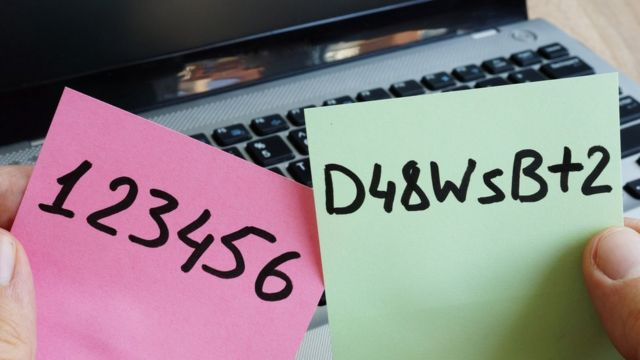
\includegraphics[scale=0.4]{img/Senha_post_it.png}
\end{figure}

Certo, precisamos então fazer uma senha segura e ter uma senha diferente para cada serviço utilizado, como lembrar então de cada senha que tenho? 

O armazenamento de senha é outro problema a ser solucionado para uma Segurança da Informação Pessoal eficiente hoje em dia. Para isso se recomenda a utilização de um programa seguro de armazenamento de senhas. Estes programas atualmente são fornecidos em diversas formas com diferentes funcionalidades, um bom exemplo é o keepass, um software que guarda e gerencia senhas utilizando criptografia para proteção com implementações em windows, linux, macOs, android e iOs. Mas também há gerenciadores de senhas integrados em navegadores de internet como Chrome ou Firefox, que também podem ser utilizados para esta função.

\section{Resumo}
Neste Capítulo aprendemos sobre as formas de acesso a uma área restrita, sendo a principal delas a senha, vimos como funcionam as senhas, como criá-las e como armazená-las. Ainda vemos como tem formas de acesso mistas e que usando isso a nossa segurança fica melhor ainda.

\chapter{Atividades}

\begin{enumerate}
\item Entre no site \href{https://www.security.org/how-secure-is-my-password/} e veja quanto tempo um hacker levaria para descobrir sua senha usando os meios que explicamos nesse capítulo e outros mais sofisticados também.
\item Faça o mesmo teste com a senha de pessoas da família e amigos, você pode até competir para ver quem tem a senha mais segura.
\item Baixe alguma versão do keepass e experimente guardar algumas de suas senhas no aplicativo.
\item Procure alguma conta sua que suporte multiplas formas de de acesso e ative mais de uma forma de acesso.
\item Acesse uma conta sua  em outro dispositivo, veja se há alguma forma de proteção automática quando você acessa sua conta em outro dispositivo.
\end{enumerate}
